There will be two main components of the user interface: the requests view (i.e. the main page), and the visual transcript view. In addition there will be a login page for the entire system. The type of user will determine exactly what content and/or interactivity is available in each view. The user type will be assessed via login credentials submitted on the login page. For example, the requests main page will give a student the option to submit a request. This page will also display any open requests and additionally it may show any closed requests that were previously completed. On the opposite side of the pipeline, faculty/admin will have a similar view showing all of the requests that require completion. Both types of users will have access to the visual transcript view which will provide an interactive visualization of the student's course history.This view will allow student users to confirm whether they meet the necessary requirements, and will allow faculty/admin to quickly identify whether a student has the necessary coursework to needed to approve the request. The faculty/admin view will contain "Approve" and "Deny" buttons which will either continue or terminate the request, respectively. Each user view is described in further detail herein. As the login page will not be a main component of the user interface, it is assumed the user has already logged in.

\begin{figure}
	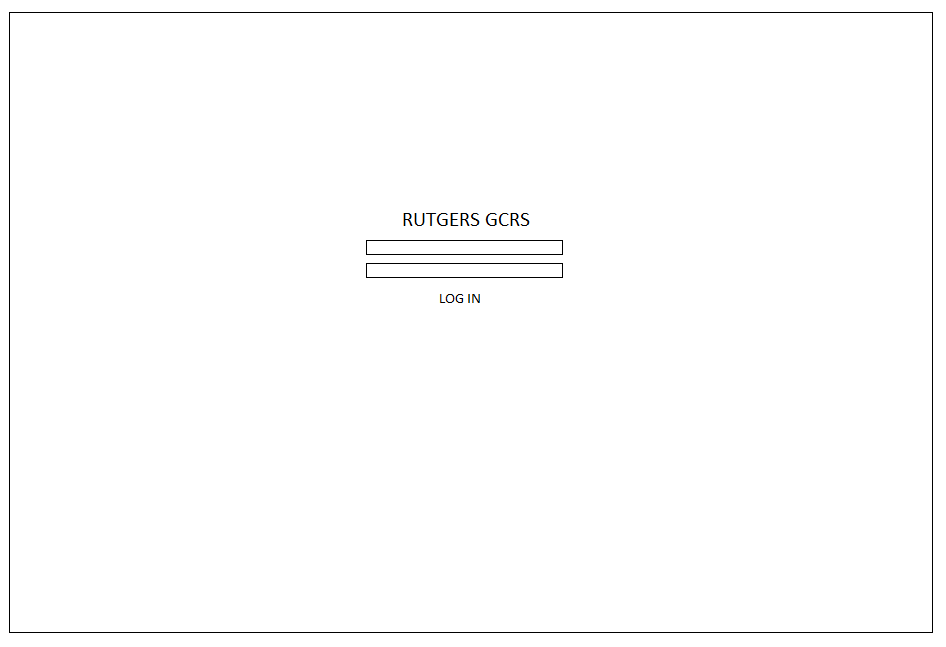
\includegraphics[width=\linewidth]{login_page.png}
	\caption{Initial Login View}
	\label{fig:fig1}
\end{figure}

For student users, the requests main page will contain a link that will take the student to their visual transcript view, and buttons to submit a new request. Any open requests will be visible in a list with options to view its status. Upon click of an open request, a window will open showing details on the status of that request. Alternatively, the status of an open request may be shown upon hover. Any closed requests (i.e. requests that were previously completed will be displayed at the bottom of the page). A wireframe representation for the requests view is given Figure 2.

\begin{figure}
	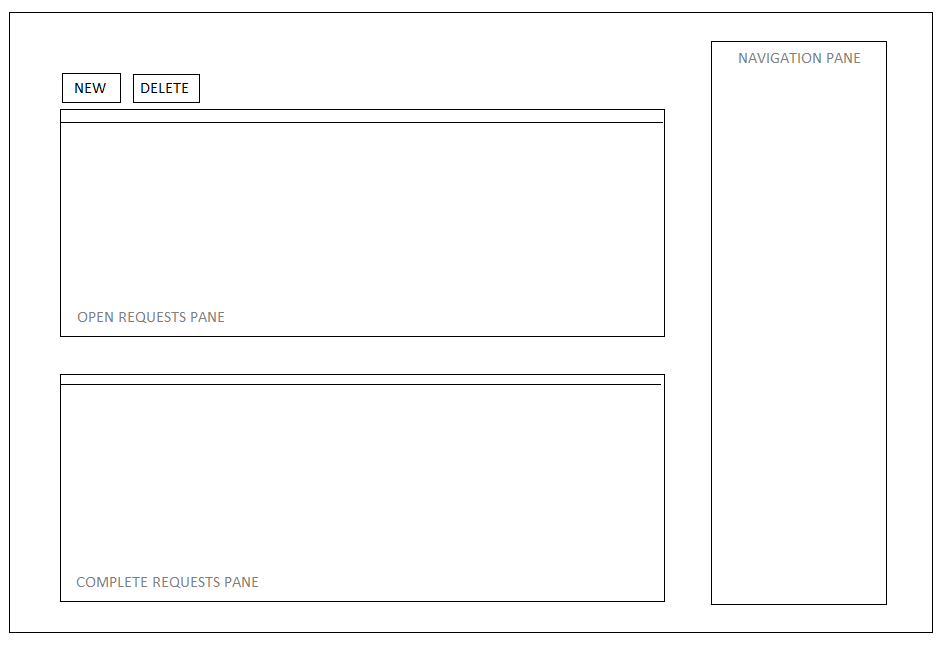
\includegraphics[width=\linewidth]{requests_main.png}
	\caption{Main Requests View}
	\label{fig:fig1}
\end{figure}

For faculty/admin users, the requests main page will appear much like the students requests page however the options available to the user will be different. In this view, faculty or admin will not require the option to submit a request. Instead all open requests (submitted by the students) will be displayed. Similar to the student view of the requests main page, the faculty/admin view will allow the user to view the status of any request and previously completed requests will be shown at the bottom of the page. The faculty/admin user will have the options to approve or deny the request (or multiple requests) from this page. The faculty/admin user will also have the option to access the students virtual transcript in order to view the students course history.

\begin{figure}
	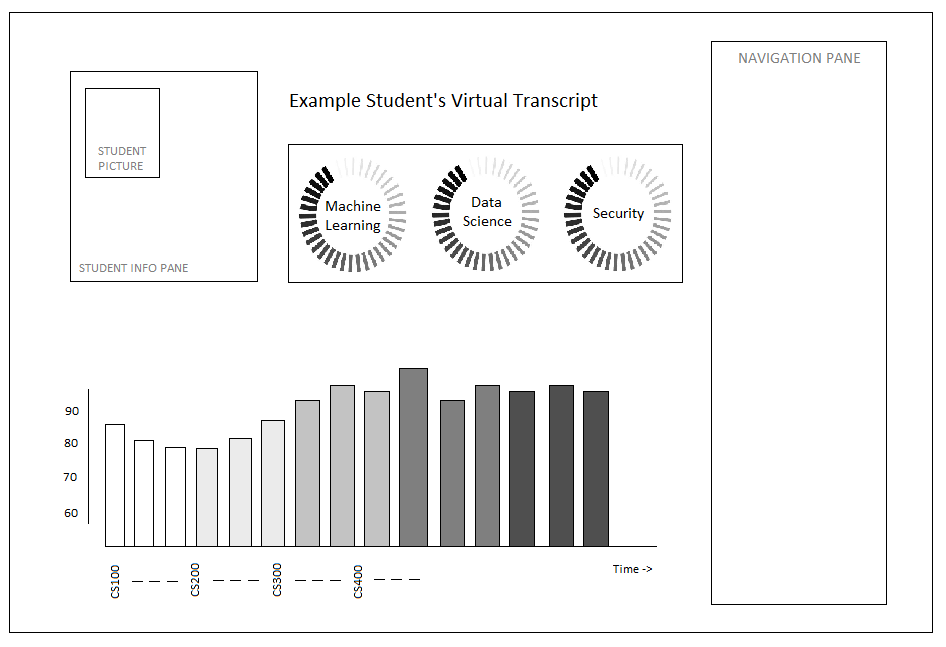
\includegraphics[width=\linewidth]{virtual_transcript.png}
	\caption{Virtual Transcript View}
	\label{fig:fig1}
\end{figure}

The purpose of this virtual transcript is to provide a visual and interactive aspect to the traditional course list and grade type transcript. This visual transcript will allow all users to quickly interpret a student's academic history. The data to be visualized in this virtual transcript will be the complete course history of the particular student as well as a visual representation of the students strengths (or weaknesses) It is imagined that the students course history will be displayed in sequential order through an adapted bar chart where the bars are located over each course and the scale of the vertical axis represents the grade the student received for the course. A color dimension will be added to represent the course level (e.g. 100, 200, 300-level courses). Additionally the students strengths and/or weaknesses in certain course concentrations (e.g. machine learning, security, data science, etc.) will be displayed via a set radial progress bars.
